\documentclass[12pt]{ociamthesis}  % default square logo 
%\documentclass[12pt,beltcrest]{ociamthesis} % use old belt crest logo
%\documentclass[12pt,shieldcrest]{ociamthesis} % use older shield crest logo

%load any additional packages
\usepackage{amssymb}
\usepackage{bbm}
\usepackage{graphicx}
\graphicspath{ {./images/} }
%input macros (i.e. write your own macros file called mymacros.tex 
%and uncomment the next line)
%\include{mymacros}

\title{Modelling and analysis of social network data from rank preferences     %your thesis title,
	}   %note \\[1ex] is a line break in the title

\author{Pierre OSSELIN}             %your name
\college{St Peter's College}  %your college

%\renewcommand{\submittedtext}{change the default text here if needed}
\degree{MSc in Mathematical Sciences}     %the degree
\degreedate{Trinity 2018}         %the degree date

%end the preamble and start the document
\begin{document}
	
	
	\maketitle                  % create a title page from the preamble info
	
	
	
	%now include the files of latex for each of the chapters etc
	\chapter{Introduction}
	This paper aims at performing inference on social network through partial ranking of the individuals
	
	
	\chapter{Community representation}
	\section{Mathematic Formulation}
	Here we suppose that the strength between individuals are characterized by their similitude to certain communities.
	
	We introduce $p$ the number of communities and $(w_{i,k})$ the strength of affiliation of the individual $i$ to the community $p$.
	
	$\lambda_{i,j} = \sum_{k = 1}^{p} w_{i,k} w_{j,k}$
	
	This formulation is equivalent to the rank matrix approximation often encountered in the literature where we assume that:
	
	$(\lambda) = WW^{T}$ where $W$ is the matrix of the $(w_{i,k})$
	
	We suppose here that the strength of the relations are only determined by the proximity with a certain community hence that the relations are reciprocal.
	
	From the reordering inequality, we can observe that $\lambda_{i,j}$ is maximized when both $i$ and $j$ have the same community ranking preferences.
	
	We can interpret the formula $\lambda_{i,j} = \sum_{k = 1}^{p} w_{i,k} w_{j,k}$ also as a scalar product in the p-dimensional space of communities. In this space, each individual is a point represented by a vector $w_{i} \in (\mathbb{R}^{+})^{p} $ the strength of affiliation is also computed by $\lambda_{i,j} = ||w_{i}||.||w_{j}||.cos(\theta)$ we can interpret the norm of the vector as the individual global influence or sociability, and the $\theta$ as the divergence in personality. Hence a given individual will appreciate another individual with great sociability but different personality or views as much as a low sociability individual with the same mindset.
	
	In this interpretation, the prior function attributed to the $w_{i,k}$ is equivalent to putting a topography on the space, allowing points to lie more likely in a certain area.
	
	In this \ref{label-image7}
	
	The main issue regarding this geometric approach is that having a bigger affiliation means that the community points have a greater scalar product, but doesn't mean those points are nearer. If we wanted to use a clustering approach to this problem, we should build a space in which the mapping to this space make it equivalent having great scalar product in the input space and being near in the output space
	
	\begin{figure}
		\centering
		%		\textbf{Your title}\par\medskip
		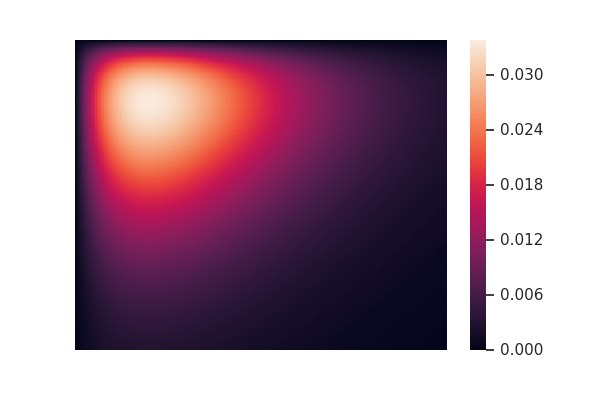
\includegraphics[width=\textwidth,height=\textheight,keepaspectratio]{heatMap}
		\caption{Topography of the community space for the same gamma distribution}
		\label{label-image7}
	\end{figure}

	\begin{figure}
		\centering
		%		\textbf{Your title}\par\medskip
		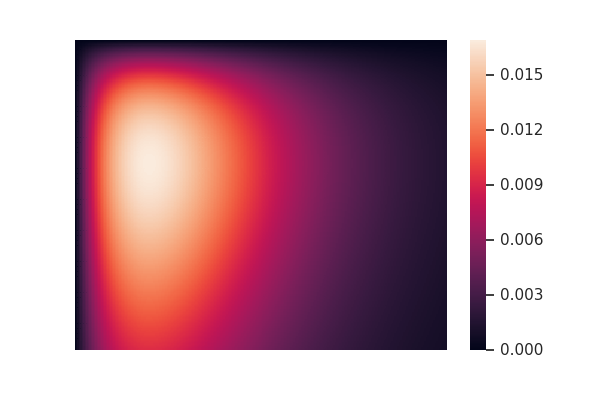
\includegraphics[width=\textwidth,height=\textheight,keepaspectratio]{heatMapCorrection}
		\caption{Topography of the community space for different gamma distribution}
		\label{label-image8}
	\end{figure}


	\section{Computation of the posterior}
	Let's define the log-posterior of the community representation. Which is the sum of the log priors of the parameters and the log-likelihood. 
	
	$l((w);D) = \sum_{i = 1}^{n} \sum_{k = 1}^{p} (\alpha - 1)ln(w_{i,k}) - \beta w_{i,k} + \sum_{i = 1}^{n} \sum_{j = 1}^{K} ln(\lambda_{i,\rho_{j}}) - ln(\sum_{j \neq i} \lambda_{i,j} - \sum_{l = 1}^{j-1} \lambda_{i,\rho_{l}})$
	
	To make the optimization easier, we can compute the gradient of the posterior according to the parameter $w_{r,s}$
	
	With $\frac{\partial \lambda_{i,j}}{\partial w_{r,s}} = 1_{i = r} w_{j,s} + 1_{j = r} w_{i,s}$
	
	We have :
	$\frac{\partial l((w);D)}{\partial w_{r,s}} = \frac{a-1}{w_{r,s}} - b 
	+ \sum_{j = 1}^{K} \frac{1}{\lambda_{r,\rho^{(r)}_{j}}} w_{\rho^{(r)}_{j},s} 
	+ \sum_{i = 1; i \neq r}^{n} \sum_{j = 1}^{K} \frac{1}{\lambda_{i,r}} w_{i,s} 1_{\rho^{(r)}_{j} = r}
	- \sum_{j = 1}^{K} \frac{1}{\sum_{j \neq r} \lambda_{r,j} - \sum_{l = 1}^{j - 1} \lambda_{r,\rho^{(r)}_{l}}} \sum_{j \neq r} w_{j,s}
	- \sum_{i = 1; i \neq r}^{n} \sum_{j = 1}^{K} \frac{1}{\sum_{j \neq i} \lambda_{i,j} - \sum_{l = 1}^{j - 1} \lambda_{i,\rho^{(i)}_{l}}} w_{i,s}$
	
	$ + \sum_{j = 1}^{K} \frac{1}{\sum_{j \neq r} \lambda_{r,j} - \sum_{l = 1}^{j - 1} \lambda_{r,\rho^{(r)}_{l}}} \sum_{l = 1}^{j-1} w_{\rho^{(r)}_{l},s}
	+ \sum_{i = 1; i \neq r}^{n} \sum_{j = 1}^{K} \frac{1}{\sum_{j \neq i} \lambda_{i,j} - \sum_{l = 1}^{j - 1} \lambda_{i,\rho^{(i)}_{l}}} \sum_{l = 1}^{j - 1} 1_{\rho^{(i)}_{l} = r} w_{i,s}$
	
	\begin{figure}
		\centering
		%		\textbf{Your title}\par\medskip
		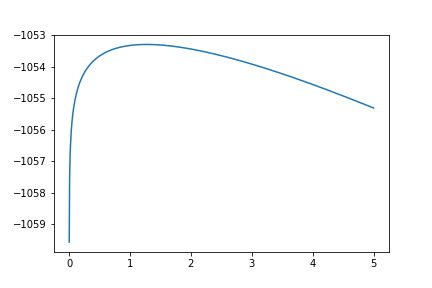
\includegraphics[width=\textwidth,height=\textheight,keepaspectratio]{CoordinateWiseFunction}
		\caption{Posterior according to one coordinate}
	\end{figure}
	
	\section{Simulations on simulated Data}
	\subsection{Fixed parameters for the prior}
	We derived two optimization algorithm to find the MAP, one based on coordinate-wise optimization, given that for the a and b considered, the log-posterior seems coordinate-wise concave, hence assuring a more stable convergence. The other algorithm is based on the L-BFGS-B algorithm, popular in machine learning optimization.
	
	For this simulation we took $a = 2$, $b = 1$ $n = 15$, $p = 3$, $k = 3$ , drew a sample from $w$, computed $\lambda$ and $\rho$. Then we maximized the posterior according to the two methods described above, in order to estimate the community strengths and then the individual mutual strength. 
%		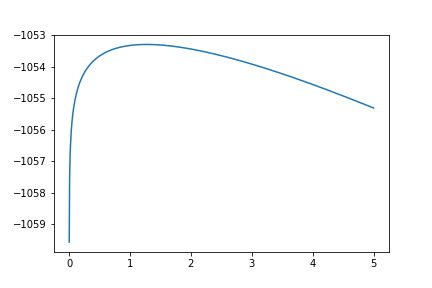
\includegraphics[width=\textwidth,height=\textheight,keepaspectratio]{CoordinateWiseFunction}

%	\begin{figure}
%		\centering
%%		\textbf{Your title}\par\medskip
%		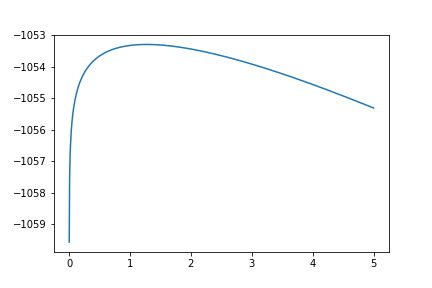
\includegraphics[width=\textwidth,height=\textheight,keepaspectratio]{CoordinateWiseFunction}
%			\caption{Posterior according to one coordinate}
%	\end{figure}

	\begin{figure}
		\centering
		%		\textbf{Your title}\par\medskip
		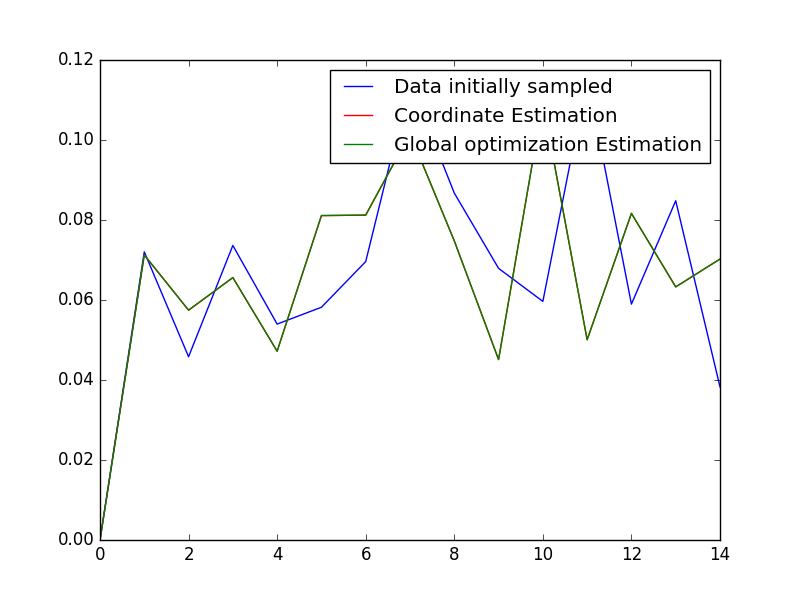
\includegraphics[width=\textwidth,height=\textheight,keepaspectratio]{LambdaEstimation}
		\caption{Comparison between the sampled and estimated Social affiliation of the first individual}
		\label{label-image1}
	\end{figure}
	
	In figure \ref{label-image1} we can see that the coordinate and global optimization have converged to the same result. We obtain an absolute error of 0.02. Which is equivalent to 0.3 reported to the number of individual, and a ranking gap (mean absolute ranking error) of 2.13 for this individual.
	
	It is interesting to compare the ranking gap to the expected ranking gap from a random permutation. We can manually compute with a tedious calculation that
	\begin{center}
		\resizebox{8cm}{!}{$ \frac{1}{n} \mathbb{E}_{\mathbb{\sigma}_{n}}[ \sum_{k = 1}^{n} |\sigma(k) - k| ] = \frac{n^{2} - 1}{3n} $}
	\end{center}
	
	For n = 18 we have a random expectation of the ranking gap of 6. Hence the model tends to preserve the "global" social network for each individual.
	
	\begin{figure}
		\centering
		%		\textbf{Your title}\par\medskip
		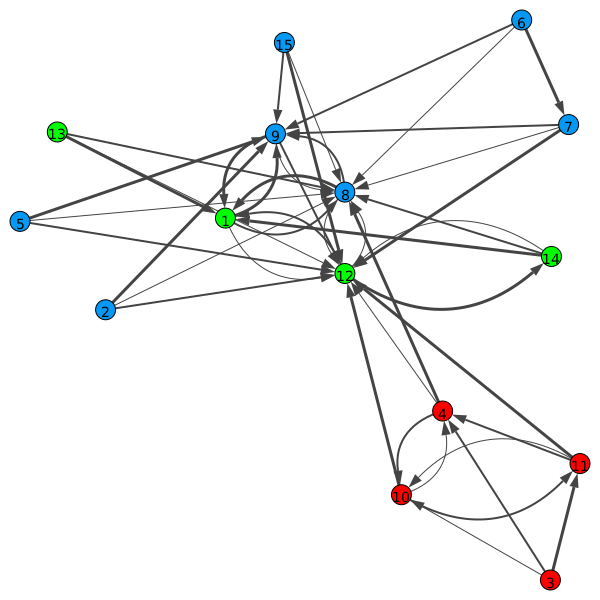
\includegraphics[width=\textwidth,height=\textheight,keepaspectratio]{OriginalPlot}
		\caption{Original Community description}
		\label{label-image2}
	\end{figure}

	\begin{figure}
		\centering
		%		\textbf{Your title}\par\medskip
		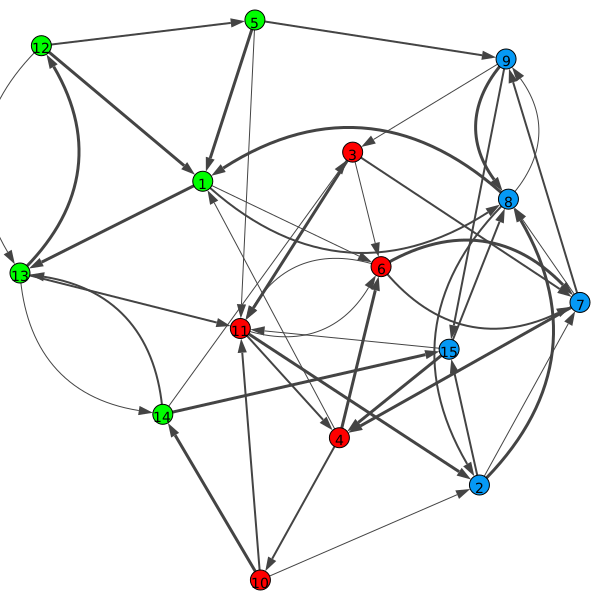
\includegraphics[width=\textwidth,height=\textheight,keepaspectratio]{OptimizationPlot}
		\caption{Inferred community}
		\label{label-image3}
	\end{figure}
	
	We can see that the inferred communities are quite similar to the original one. The original red and green communities are preserved except for the individual 6 and 5 that has passed from the blue community to the red and green respectively. Here we have assigned an individual to his preferred community, the width of an edge represents the importance the son represents for the father.
	\subsection{Model with degree-correction}
	
	In this subsection, we try to capture the different popularity that a community can have over the other communities. In the previous model, the regularization terms $w_{i,j}$ in the posterior had the same weights, irrespective of the community concerned (Having a too big $w_{i,j}$ was equally improbable regardless of the community). In a model with degree-correction, i.e in which $w_{i,k} \sim  \Gamma(\alpha, \beta_{k})$, we do not prevent the possibility of a popular community in the regularization, which occurs by the emergence of popular individuals.
	\begin{figure}
		\centering
		%		\textbf{Your title}\par\medskip
		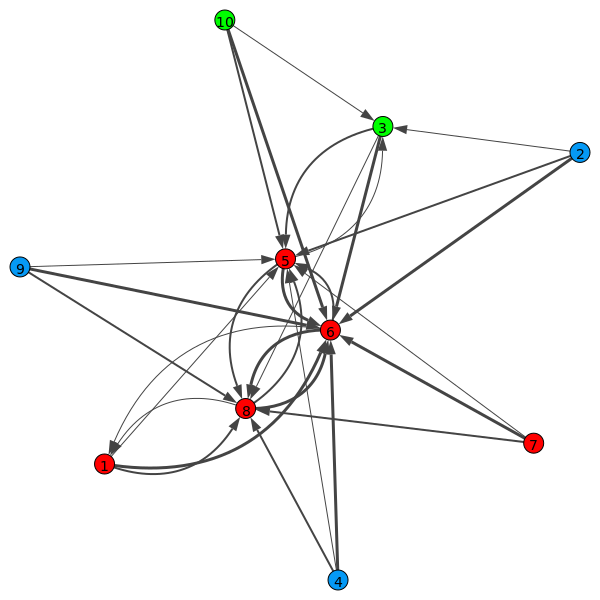
\includegraphics[width=\textwidth,height=\textheight,keepaspectratio]{OriginalPlotDegreeCorrection}
		\caption{Original Community description for the degree Correction Model}
		\label{label-image5}
	\end{figure}
	
	\begin{figure}
		\centering
		%		\textbf{Your title}\par\medskip
		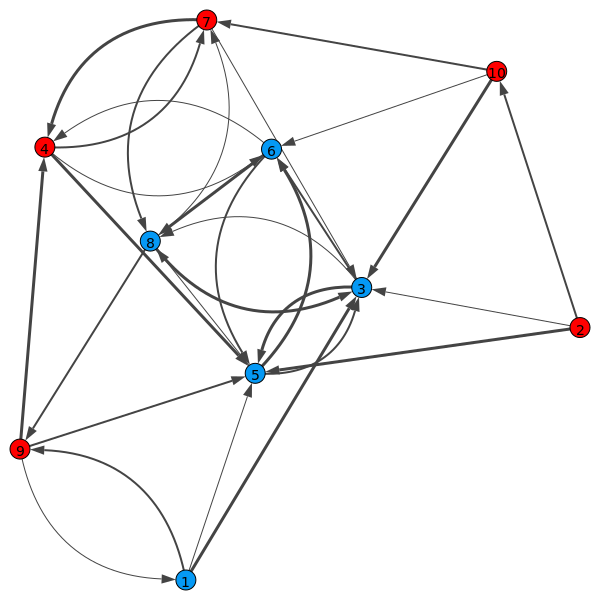
\includegraphics[width=\textwidth,height=\textheight,keepaspectratio]{OptimizationPlotDegreeCorrection}
		\caption{Inferred community for the degree correction Model}
		\label{label-image6}
	\end{figure}
	
	
	We can see in this example that the green community has been absorbed in an other community by the inference, and that 7 has been replaced by 3 in the other community.
	
	\subsection{Performance Comparison}
	
	To evaluate the performance of the models, we make prediction on the preferences for individuals who have not indicated their preferences, provide further preferences from individuals who did, or extract from the lists interpretable information about the structure of the underlying friendship network, e.g. in terms of latent communities. For this we will use different metrics. The ranking gap between latent appreciation, the absolute error in the strengths and the missed community. To do that, we will sample the strengths between individuals $\lambda_{i,j}$ and then sample full rankings from it. From this ranking we then hide a certain part of it, we feed the remaining parts to our model and then compute the error in terms of metrics previously defined to evaluate the performance.
	
	\section{Model with Covariates}
	
	The purpose of ERGMs, in a nutshell, is to describe parsimoniously the local selection forces
	that shape the global structure of a network. To this end, a network dataset, like those
	depicted in Figure 1, may be considered like the response in a regression model, where the
	predictors are things like “propensity for individuals of the same sex to form partnerships” or
	“propensity for individuals to form triangles of partnerships”. In Figure 1(b), for example, it
	is evident that the individual nodes appear to cluster in groups of the same numerical labels
	(which turn out to be students’ grades, 7 through 12); thus, an ERGM can help us quantify
	the strength of this intra-group effect. The information gleaned from use of an ERGM may
	then be used to understand a particular phenomenon or to simulate new random realizations
	of networks that retain the essential properties of the original. Handcock, Hunter, Butts,
	Goodreau, and Morris (2008) say more about the purpose of modeling with ERGMs; yet in
	this article, we focus primarily on technical details.
	
	\subsection{Notation}
	Let $N$ be the set of nodes in the network of interest, indexed $\{ 1,...,n\}$ The relationships in
	the network may be directed (e.g., friendship nominations, messages) or undirected (e.g., sexual
	partnerships, conversations). In the former case, we define the set of dyads (here used to refer
	to potential relationships) $\mathbb{Y}$ to be a subset of $N \times N$, the set of ordered pairs of nodes; in the
	latter case, it is a subset of $\{ \{i, j\} : (i, j) \in N \times N\}$, the unordered pairs of nodes. (We will also
	use u($\mathbb{Y}$) to refer to an “unordered” version of $\mathbb{Y}$, i.e., u($\mathbb{Y}$) $\equiv$ $\{\{i, j\} : (i, j) \in Y \}$.) Usually, $\mathbb{Y}$ is
	further constrained in that in most social networks studied, a node cannot have a relationship of
	interest with itself, excluding pairs of the form $(i, i)$.
	For binary networks, in which the relationship of interest must be either present or absent,
	we use $\mathcal{Y}$ $\in$ $2^{\mathbb{Y}}$
	, the set of subsets of $\mathbb{Y}$, to refer to the set of possible networks of interest, which may be further constrained (that is, $\mathbb{Y}$ may be a proper subset of $2^{\mathbb{Y}}$). We will use $\textbf{Y}$ to refer to
	network random variables and $y$ $\in$ $\mathcal{Y}$ to refer to their realizations, and $y_{i,j}$ be an 0 - 1 indicator of
	whether a relationship of interest is present between i and j in a binary network context.
	
	
	\subsection{ERGM model}
	In the ERGM model (exponential-family random graph models), the distribution of $\textbf{Y}$ can be parameterized in the form:
	
	\resizebox{7cm}{!}{$P_{\theta}(Y = y) = \frac{exp((\eta(\theta)) ^{T}*z(x))}{\chi(\theta)}, y \in \mathcal{Y}$}
	
	where $\theta$ is a q-vector of model parameters, which are mapped to a p-vector of natural parameters
	by $\eta(.)$, and $g(.)$ is a p-vector of sufficient statistics, which capture network features of interest. These sufficient statistics typically embody the
	features of the network of interest that are believed to be significant to the social
	process which had produced it, such as degree distribution (e.g., propensity
	towards monogamy in sexual partnership networks), homophily (i.e., “birds of
	a feather flock together”), and triad-closure bias (i.e., “a friend of a friend is a
	friend”) . (Morris, Handcock and Hunter, 2008)
	
	\subsection{The p1 Model}
	
	The $p_{1}$ model is the first to propose log-linear models for social
	networks. Suppose that we take Y to be the set of all directed graphs, with independent dyads [i.e., the pairs (Y ij , Y ji ) are independent for different choices of {i, j}] and the following model for tie probabilities:
	
	1) 
	1) ERGM models
	2) Bernouilli model
	3) p1 Model
	4) 
	
	ERGM models • As described, models work very poorly
	• Learned parameters do not generate data that resembles the input
	• Tend toward wholly connected or completely empty graphs
	
	
	
	
	
	
	
	
	
	
	
	
	
	P1 Model : Original exponential family graph, with dyadic independence (facilitate the expression of the likelihood) and $P(Y_{i,j} = y_{1}, Y_{j,i} = y_{2}) \propto exp\{  y_{1}(\mu + \alpha_{i} + \beta_{j}) + y_{2}(\mu + \alpha_{j} + \beta_{i}) + y_{1}y_{2}\rho \}   $
	
	
	Problem : Model degeneracy had proposed tend to, as the network size increases, concentrate an increasingly
	large probability mass on an increasingly small fraction of possible networks.
	
	Models based on independence conditional on latent
	variables: random
	effects models and mixed effects models and extensions; stochastic block models and extensions,
	including mixed membership models; and latent space models and extensions.
	
	Assume dyads conditional independent given some latent variables. i.e
	$P_{\theta}(Y = y | Z = z) = \prod_{(i,j) \in u(\mathbb{Y})} P_{\theta}(Y_{i,j} = y_{i,j}, Y_{j,i} = y_{j,i} | Z = z)$ Except the p2 model, we even assume $Y_{i,j}$ and $Y_{j,i}$ independant given $Z$.
	Those models can capture network dependencies of interest and are easier to work with in terms of computation.
	
	Paper studied uses p2 model and add in a likelihood that take ranking into account. And compare it to other likelihood that do not and compare and draws conditions in wich ranking provide information.
	
	
	
	These sufficient statistics typically embody the
	features of the network of interest that are believed to be significant to the social
	process which had produced it, such as degree distribution (e.g., propensity
	towards monogamy in sexual partnership networks), homophily (i.e., “birds of
	a feather flock together”), and triad-closure bias (i.e., “a friend of a friend is a
	friend”) . (Morris, Handcock and Hunter, 2008)
	A major limitation of ERGMs to date has been t
	
	
	\subsection{Random effects and mixed effects models}
	p2 modelp1 model can be
	represented as a generalized linear model and the p2 model as a generalized linear mixed model
	
	
	\subsection{Stochastic block models}
	
	\subsection{Latent space models}
	
	\section{Simulations on the Sampson’s monk dataset}
	In this part we use the The data set collected by Sampson (1968) this is a classic data set in social network analysis. The data set summarizes relationships, observed at three distinct time points, among 18 monks who were about to enter a monastery when a conflict erupted. We use here the directed network where $y_{i,j} = 1$ denotes that monk i ranked monk j among his top three preferred individuals and $y_{i,j} = 0$ otherwise. The directed network is shown in Figure \ref{label-image4} , where circles represent monks and directed edges are oriented from i to j whenever $y_{i,j} = 1$. The monks are divided by Sampson into three groups: Loyal Opposition, Turks, and Outcasts.
	
	We applied the same method as for the simulated data and obtained the following community. We can observe that our model identifies exactly the same clustering of communities as the ones observed by Sampson. Namely the Loyal Opposition (Red community), Turks (Green Community), and Outcasts (Blue Community). In this graph the individuals are labeled according to their number provided with their names in the data set package and not according to their rank in the data-frame.
	
	
	\begin{figure}
		\centering
		%		\textbf{Your title}\par\medskip
		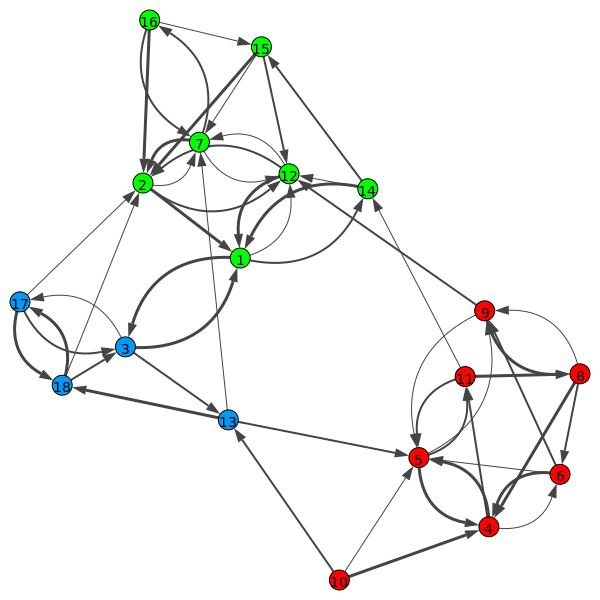
\includegraphics[width=\textwidth,height=\textheight,keepaspectratio]{OptimizationPlotSam}
		\caption{Inferred community for the Sampson DataSet}
		\label{label-image4}
	\end{figure}
	
	
	
\end{document}